%************************************************
\chapter{Design and Implementation}\label{ch:implementation} % $\mathbb{ZNR}$
%************************************************
\glsresetall % Resets all acronyms to not used

In this chapter it is explained in detail how NEAT and ns-3 were modified from a technical view. At first we look into the general functioning of NEAT-TCP and how it is organised. Then we look deeper into the implementation and the encountered hurdles and how they are mastered.

\section{NEAT-TCP Design and Concept}\label{sec:neatOrganisation}

The organisation of NEAT-TCP is visualised in \autoref{fig:technicalNEATorga}. There it can be seen that \texttt{NEAT::Experiments} is the entry point of the algorithm. Actually on top of it is \texttt{Neatmain}, but 
this class only selects the experiment to start and thus has no real influence on NEAT-TCP. Also in \autoref{fig:neatIteration} the functioning in a finite state diagram is visualised. The following refers to both figures.
\begin{center}
\begin{figure}
	\centering
	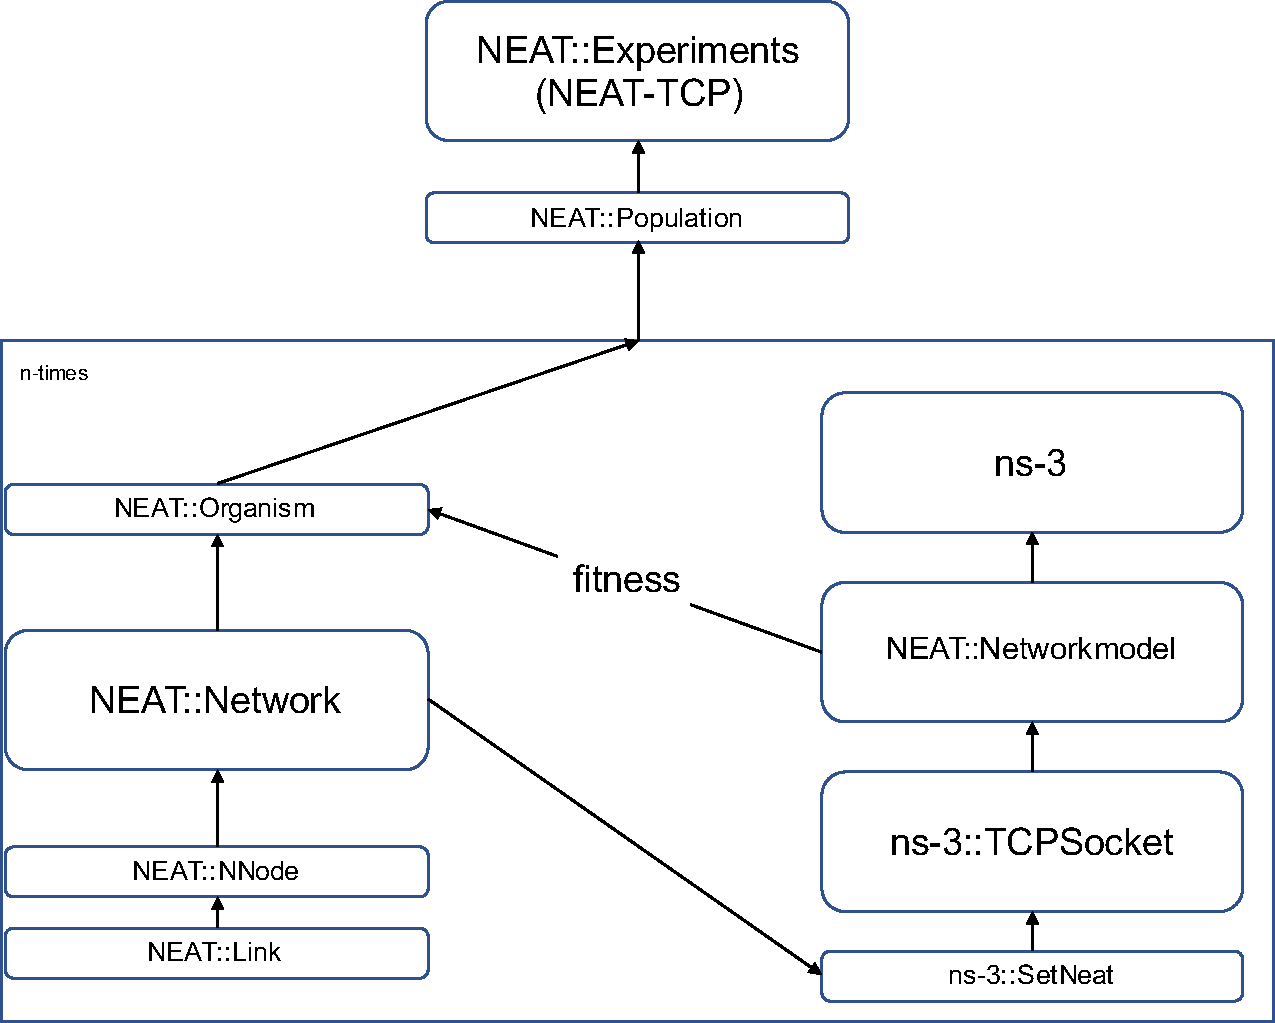
\includegraphics[scale=0.5]{technicalNEATorga}
	\caption{Visualisation of the implementation of NEAT}
	\label{fig:technicalNEATorga}
\end{figure}
\begin{figure}
	\centering
	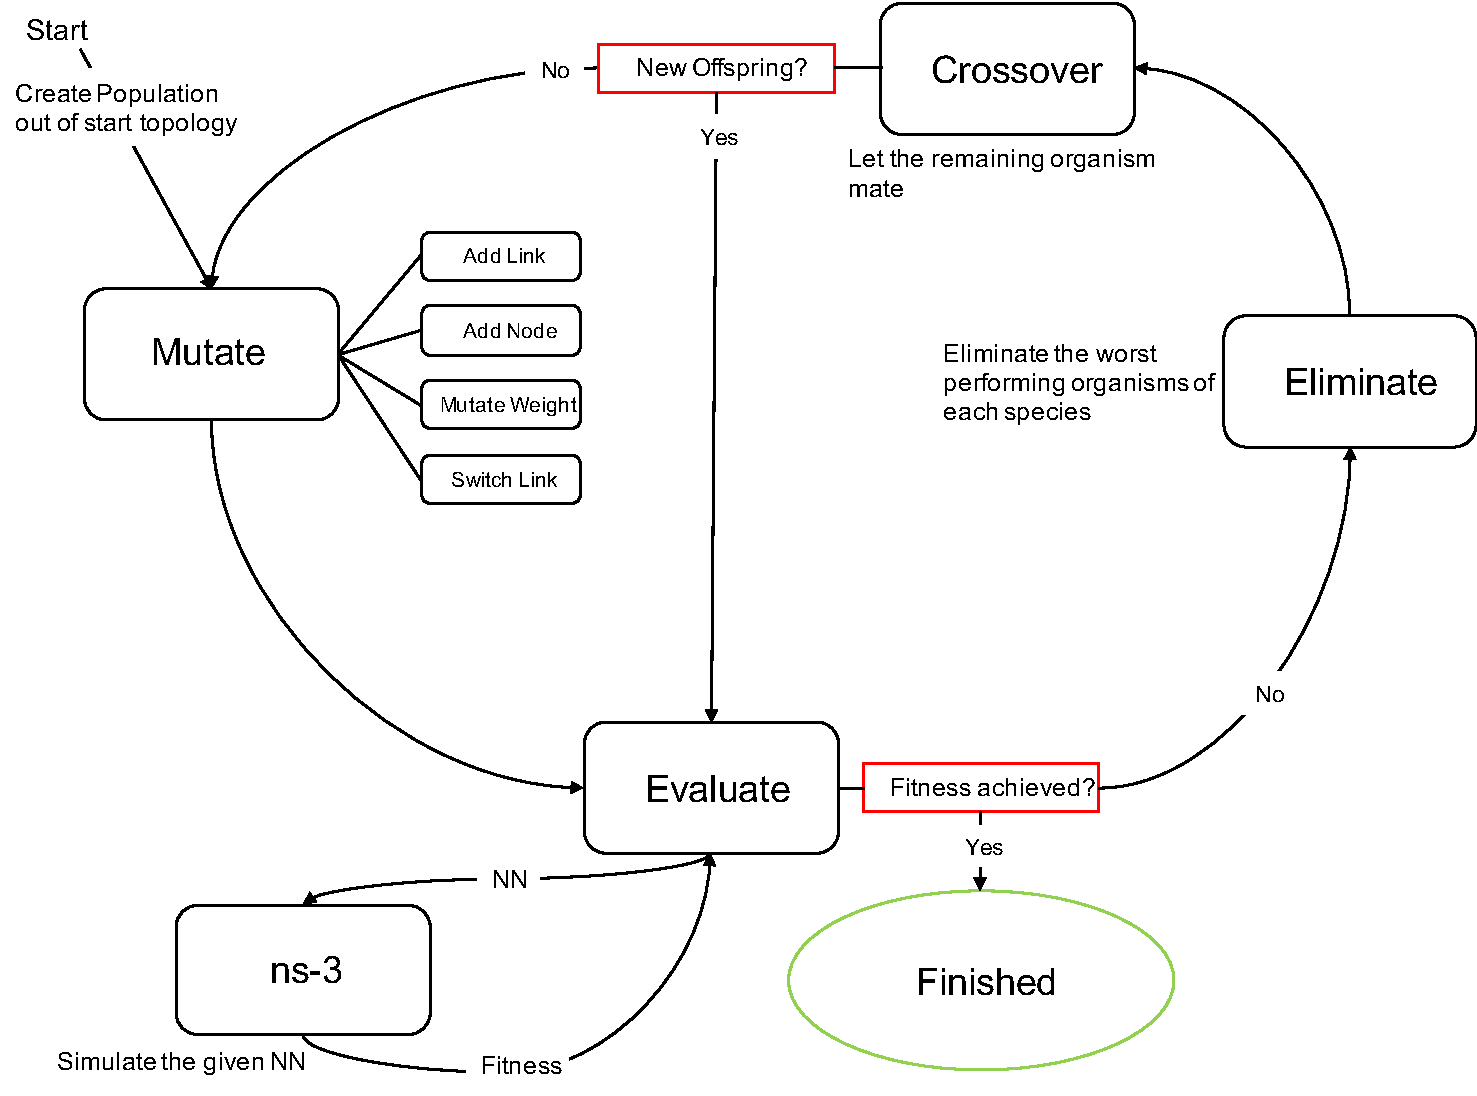
\includegraphics[scale=0.5]{neatIteration}
	\caption{Visualisation of the operation of NEAT}
	\label{fig:neatIteration}
\end{figure}
\begin{figure}[h]
	\centering
	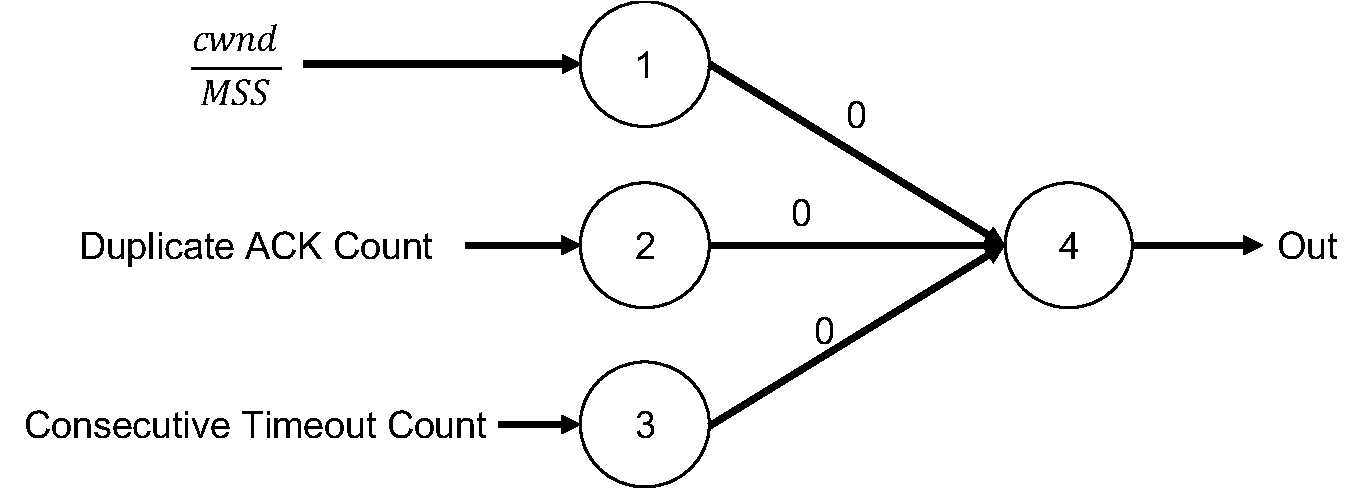
\includegraphics[width=1\linewidth]{neatTCPstart}
	\caption{NEAT-TCP initial neural network}
	\label{fig:neatTCPstart}
\end{figure}
\end{center}

NEAT-TCP starts by reading a parameter file and then creating a population of organisms accordingly. These organisms are neural networks that are only connecting the inputs and outputs with a link weight of 0. The start NN has to be specified in a separate file named \texttt{ccstartgenes}. The NEAT paper states that the start NN should be of this structure, because this makes it more likely to get a minimal result \cite{neat}. In \texttt{NEAT::Organism}, the genotype, phenotype, fitness and other parameters of a NN are saved. The genotype is the genetic encoding of the neural network and the phenotype is the structure of the neural network that results from its genotype. \\
After creating the population the evolution begins with mutating it, with the chances and intensities provided in the parameter file. The possible mutations are mentioned in \autoref{sec:mutation}. Then the fitness of the organisms is evaluated. For that, each phenotype is passed to the \texttt{NEAT::Networkmodel}, where the \gls{WMN} is specified. The WMN is further described in \autoref{subsec:networkspec}. In the WMN each TCP socket is initialised explicitly and the neural network is passed through. So each TCP Socket has the same NN for themselves. 
Then the network is simulated and the achieved fitness is returned, set in \texttt{NEAT::Organism} and if the fitness is above the targeted fitness, it is also marked as a winner. The evaluation has to be done for every organism in the population independently. \\
After the population is evaluated, it is checked if there are any winners. If there are, the evolution is over. If not it continues by speciating the population, further described in \autoref{sec:speciation}. Then the worst performing organisms of each species get eliminated. The parameters of the parameter file define how many get eliminated. Now that there is some room for new organisms, since the population size has to be constant, NEAT-TCP allows the population to mate. After that, the population mutates again if it is not just born.  Crossover, elimination, speciation and mutation are implemented in \texttt{NEAT::Population}. \\
The NN of NEAT-TCP works with the same inputs as iTCP, namely the congestion window divided by the maximum segment size, duplicate ACK count and the consecutive timeout count, and its initial neural network is visualised in \autoref{fig:neatTCPstart}.



\section{Integration of NEAT-TCP into ns-3}\label{sec:extensionns3}
To use NEAT-TCP the NNs need to be passed to the nodes of the WMN. To get the local features for the inputs of the NNs, we set the \texttt{NEAT::Network} objects, that are created by the NEAT algorithm and inherit the NNs, directly on the socket. 
So the socket needs to be accessed directly in the \texttt{NEAT::Networkmodel}. This is not possible if there are applications that were created by their associated helpers, as their socket is not accessible. In this work we first created the sockets and then passed them to a custom application without a helper. \\
In the following, the implementation and challenges that come with it are further described.

\subsection{TCP Structure in ns-3}\label{subsec:tcpstruct}
Briefly, TCP sockets in ns-3 are structured like in \autoref{fig:TcpSocket}. In the center is \texttt{TCP-Socket-Base} with all functions that TCP needs to operate. \texttt{TCP-Congestion-Ops} is the congestion control algorithm that can be set in \texttt{TCP-Socket-Base}. In this file TCP New Reno is specified and all other TCP flavours inherit this class. One would guess to just implement NEAT-TCP in \texttt{TCP-Congestion-Ops} or extend it, but this is not possible. Although congestion control algorithms are extending this file, in the simulation or when building the topology there is no possibility of passing an object, like the NN, to this algorithm and then giving it to the socket. Also \texttt{TCP-Socket-Base} would call functions of the specified congestion control algorithm if it thinks the congestion window should be increased. Then it calls the \texttt{IncreaseWindow} function or when a packet is acknowledged the \texttt{PktsAcked} function. Because no object can be passed to \texttt{TCP-Congestion-Ops}, NEAT-TCP is implemented on \texttt{TCP-Socket-Base} so a \texttt{NEAT::Network} can be easily passed through. \\
Another problem with the structure of ns-3 is the application handling. When creating an application a helper needs to be called which sets the wanted application. By this method it may be easier to create these applications, but with doing it that way the socket the application is working with cannot be accessed directly, which means that the \texttt{NEAT::Network} cannot be set for these applications. To use NEAT-TCP, the socket has to be created first, then the \texttt{NEAT::Network} has to be set and then the socket can be passed to an application.


\subsection{Changes to ns-3 TCP}
\begin{figure}[h]
	\centering
	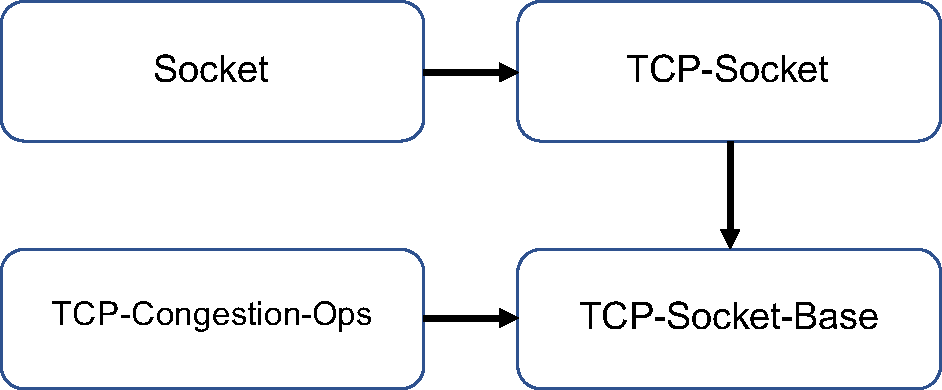
\includegraphics[width=1\linewidth]{Tcp-Socket}
	\caption{Inheritance diagram of TCP socket in ns-3}
	\label{fig:TcpSocket}
\end{figure}
At first \texttt{Socket}, \texttt{TCP-Socket} and \texttt{TCP-Socket-Base} are extended by a virtual setter function that accepts a \texttt{NEAT::Network} as its only parameter. The virtual setter function has to also be defined in \texttt{Socket} and \texttt{TCP-Socket}, because when creating a TCP socket it creates a \texttt{Socket} object which is extended by the other classes and only the functions that are defined in the \texttt{Socket} can be accessed. By extending these two classes with these functions, a \texttt{NEAT::Network} can be passed to \texttt{TCP-Socket-Base} and saved there. \texttt{TCP-Socket-Base} has to be changed in such a way that it does not call \texttt{TCP-Congestion-Ops} anymore. Rather it needs to activate the \texttt{NEAT::Network} of NEAT-TCP, which will be described in \autoref{subsec:neatuse}. \\ Further, NEAT-TCP needs a counter of consecutive timeouts as one of its inputs, which is not given. This counter is defined in \texttt{TCP-Socket-Base} because the timeout functions are defined there, which need to increment this counter and if a packet is received this counter needs to be set to 0 again. The other input, which is the duplicate ACK count, is already implemented in ns-3.\\
There is a technical problem in doing it that way. All those classes need to import the \texttt{network} file from NEAT, where the neural network object is defined, which is located in the \texttt{scratch} folder of ns-3. This folder is not included while compiling these files, which is why the \texttt{wscript} files need to be modified. Ns-3 uses the \textit{waf} compiler which uses these \texttt{wscripts} to define what has to be included in the compilation. In ns-3, every folder has a \texttt{wscript}. In this case the paths to the NEAT \texttt{network} files have to be added to the \texttt{wscript} of the \texttt{Internet} and \texttt{Network} folder.


\section{NEAT Implementation}\label{sec:neatimpl}
The original implementation of NEAT is not used in this work. Rather a tidied up version \cite{neatimpl} created by GitHub user FernandoTorres is used. The reason for this is that it works the same, while being easier to understand and work with. In the following it is described how this implementation of NEAT is extended and modified to be able to run within ns-3 and generate NEAT-TCP.

\subsection{NEAT Usage in ns-3}\label{subsec:neatuse}
The used NEAT implementation uses the file extension \texttt{.cpp}. In this work NEAT is located in the \texttt{scratch} folder. The \texttt{scratch} folder is the main location for custom experiments in ns-3. The network simulator ns-3 solely uses \texttt{.cc} for its files, which is why either all files of this implementation need to be changed to \texttt{.cc} or it has to be specified in the \texttt{wscript} of the root directory of ns-3 that it has to read \texttt{.cpp} files within the \texttt{scratch} folder. In this work all file extensions of the NEAT implementation are changed to \texttt{.cc}, because this way it can be adopted more easily. \\\\
In that way, NEAT is handled just like any other custom ns-3 network module. \\
To evaluate the \texttt{NEAT::Network} several inherited functions must be called. At first the input layer needs to be loaded with the current values. After that it has to be activated with the \texttt{activate} function. Then the activation of the outputs can be read. Also, if the NN is recurrent, the values are saved in \texttt{NEAT::Network} and then used within the next activation.

\subsection{Extending NEAT to NEAT-TCP}
The used NEAT implementation includes some example code to demonstrate possible fields of applications: the evolution of an XOR gate, balancing a single pole or two poles with velocity information and balancing two poles without velocity information provided on a two dimensional moving cart. In the \texttt{neatmain} file the choice for NEAT-TCP needs to be added so it can be executed. Further, all experiments are located in the \texttt{experiments} file. There the NEAT-TCP experiment is added. It is basically the XOR experiment but with a slightly different evaluation. Wheras the XOR networks would be fed four different input sets and then be evaluated on all these by subtracting the outputs from the wanted results, NEAT-TCP networks need to be evaluated within the ns-3 network simulation. At first there is a network file needed in which the communication network is specified. In \autoref{subsec:networkspec} it is described in detail how the network is specified. All genomes in the population need to be tested in the ns-3 simulation. That are a lot of simulations, which raises the question for parallelisation. The problems that come with it and how they can be dealt with are described in \autoref{subsec:parallelisation}. The fitness of each NEAT-TCP network is calculated in the \texttt{experiments} file and the \texttt{network} file returns a vector containing the measures of the simulation to it.  There are no further changes needed to be made to NEAT to execute NEAT-TCP. Because the evaluation loop is executed in every generation and evaluates every network with a simulation, which takes a lot of computing time, we look into parallelisation in the next section.

\subsection{Parallelisation}\label{subsec:parallelisation}
There are two ways NEAT-TCP could be parallelised. Either (i) parallelise the evaluation loop or (ii) parallelise the simulation itself. Since ns-3 generally only runs on a single thread, the first way would theoretically result in an n-times reduction in run time, where n is the number of threads.  The second way has shown to be not effective. The MPI framework that is included and well documented in ns-3 allows to allocate certain nodes to certain threads. Since in this work 25 nodes are used, it is intuitive to at least allocate 5 nodes to one thread each and let 3 threads do coordination work. Unfortunately it is shown that our scenario, described in more detail in \autoref{sec:expsetup}, would not benefit from the wanted run time decrease \cite{distributedns3}. \\\\
For the first approach OpenMP \cite{openmp} was used. OpenMP allows for easy parallelisation of \texttt{for} loops. There is native support for it in the g++ compiler when the flag \texttt{-fopenmp} is set. The evaluation loop was parallelised with the parallel command but it caused errors within ns-3. There are two files within the core of ns-3 that assert that the thread they were executed in is the original thread the simulation has been started in, namely in \texttt{default-sim-impl.cc} at line 299 and in \texttt{simple-ref-count.h} at line 103. Commenting out these asserts resulted in memory errors. The reason could be that ns-3 treats the whole NEAT execution as one simulation and not as a simple program that is starting multiple different simulations at once. Ns-3 may not be thread safe, which means that in the current state of ns-3 it is not possible to speed up NEAT-TCP. But in general NEAT is able to be parallelised, which means that if a thread safe network simulator is used, the run time of NEAT-TCP would be vastly reduced.

\section{iTCP Implementation in ns-3}\label{sec:itcpimpl}
\begin{figure}[h]
	\centering
	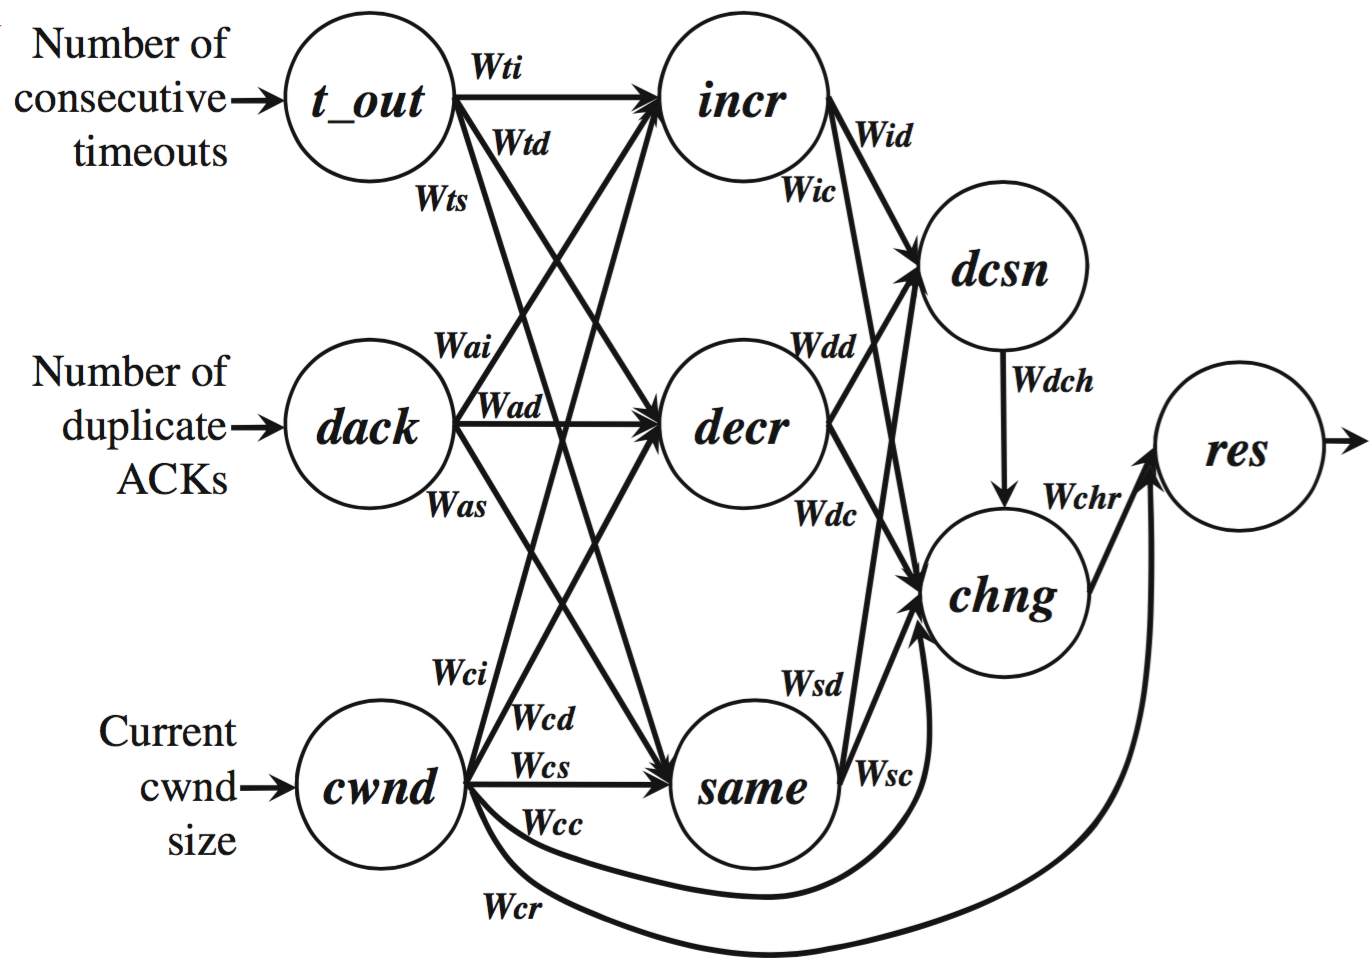
\includegraphics[width=1\linewidth]{itcp}
	\caption{Neural network of iTCP \cite{iTCP}}
	\label{fig:itcp}
\end{figure}
iTCP is a feedforward neural network for congestion control, that uses various different activation functions. 
All nodes have a unique activation function, besides the nodes on the input layers. 
The link weights are constant throughout the operation, so iTCP is a reinforcement learned neural network, and not a reinforcement learning based neural network.
\\Since iTCP uses various activation functions, it can not be built as a \texttt{NEAT::Network} object. 
NEAT is not made to be used with various activation functions within the same network and has no support for it. 
In theory NEAT could be extended to be able to use various activation functions but this would result in a new kind of mutation that would also have to be added. 
But this is not a problem since the iTCP neural network is static and not recurrent.
It is implemented explicit within \texttt{tcp-socket-base}.
 All activation functions are explicitly implemented there as well. 
The neural network of iTCP is evaluated every time a packet is acknowledged.\\ 
We asked the developers of iTCP for their source code, because there were some ambiguities in their paper. 
So we received a ns-2 implementation of iTCP which resolved these ambiguities. 
The TCP socket has a completely different structure in ns-2 than in ns-3. 
For example the congestion window is a number that describes how many segments can be sent, whereas in ns-3 the congestion window is the number of bytes that can be sent.
iTCP has a maximum which has to be set and the authors described for one of their experiments, with less transmission rate than in our network \autoref{subsec:networkspec}, that it was set to 128, so at maximum 128 segments can be sent. 
If implemented the same way in ns-3, it would mean that 128 bytes can be sent at maximum, which is about a quarter of a segment so not a single segment could be sent. 
However, the neural network of iTCP can be used with only slight changes of the ns-2 code in ns-3. 
The only change to be made is to set the maximum value, or to provide the neural network the number of segments by dividing the congestion window by the segment size.
In \autoref{ch:evaluation}, we evaluate both implementations. iTCP that is fed the congestion window in byte with a maximum of 2680 bytes is further called \textit{iTCP-bytes}. And iTCP that is fed the congestion window as the number of segments with a maximum of 5, like in the iTCP paper is further called \textit{iTCP-seg}. \\
We tried several different maxima for \textit{iTCP-bytes} and found out that the maximum has influence on the convergence and fairness. For maxima above 2.680 bytes, we observed no difference in behaviour. If the maximum was below 2680 bytes (5 segments), iTCP would have no influence on the performance and the congestion window could be set to this permanently, because our network model \autoref{subsec:networkspec} is capable of sending with a congestion window of 3 without congestion. 
Also \textit{iTCP-seg} effectively never reaches its maximum in practical experiments, yet it was specified like this in the iTCP paper \cite{iTCP}.